% 2-5-solving-recurrence.tex

%%%%%%%%%%%%%%%%%%%%
\documentclass[a4paper, justified]{tufte-handout}
\usepackage{graphicx}
\usepackage[outdir=./]{epstopdf}

% hw-preamble.tex

% geometry for A4 paper
% See https://tex.stackexchange.com/a/119912/23098
\geometry{
  left=20.0mm,
  top=20.0mm,
  bottom=20.0mm,
  textwidth=130mm, % main text block
  marginparsep=5.0mm, % gutter between main text block and margin notes
  marginparwidth=50.0mm % width of margin notes
}

% for colors
\usepackage{xcolor} % usage: \color{red}{text}
% predefined colors
\newcommand{\red}[1]{\textcolor{red}{#1}} % usage: \red{text}
\newcommand{\blue}[1]{\textcolor{blue}{#1}}
\newcommand{\teal}[1]{\textcolor{teal}{#1}}

\usepackage{todonotes}

% heading
\usepackage{sectsty}
\setcounter{secnumdepth}{2}
\allsectionsfont{\centering\huge\rmfamily}

% for Chinese
\usepackage{xeCJK}
\usepackage{zhnumber}
\setCJKmainfont[BoldFont=FandolSong-Bold.otf]{FandolSong-Regular.otf}

% for fonts
\usepackage{fontspec}
\newcommand{\song}{\CJKfamily{song}} 
\newcommand{\kai}{\CJKfamily{kai}} 

% To fix the ``MakeTextLowerCase'' bug:
% See https://github.com/Tufte-LaTeX/tufte-latex/issues/64#issuecomment-78572017
% Set up the spacing using fontspec features
\renewcommand\allcapsspacing[1]{{\addfontfeature{LetterSpace=15}#1}}
\renewcommand\smallcapsspacing[1]{{\addfontfeature{LetterSpace=10}#1}}

% for url
\usepackage{hyperref}
\hypersetup{colorlinks = true, 
  linkcolor = teal,
  urlcolor  = teal,
  citecolor = blue,
  anchorcolor = blue}

\newcommand{\me}[4]{
    \author{
      {\bfseries 姓名:}\underline{#1}\hspace{2em}
      {\bfseries 学号:}\underline{#2}\hspace{2em}\\[10pt]
      {\bfseries 评分:}\underline{#3\hspace{3em}}\hspace{2em}
      {\bfseries 评阅:}\underline{#4\hspace{3em}}
  }
}

% Please ALWAYS Keep This.
\newcommand{\noplagiarism}{
  \begin{center}
    \fbox{\begin{tabular}{@{}c@{}}
      请独立完成作业,不得抄袭。\\
      若得到他人帮助, 请致谢。\\
      若参考了其它资料,请给出引用。\\
      鼓励讨论,但需独立书写解题过程。
    \end{tabular}}
  \end{center}
}

\newcommand{\goal}[1]{
  \begin{center}{\fcolorbox{blue}{yellow!60}{\parbox{0.50\textwidth}{\large 
    \begin{itemize}
      \item 体会``思维的乐趣''
      \item 初步了解递归与数学归纳法 
      \item 初步接触算法概念与问题下界概念
    \end{itemize}}}}
  \end{center}
}

% Each hw consists of four parts:
\newcommand{\beginrequired}{\hspace{5em}\section{作业 (必做部分)}}
\newcommand{\beginoptional}{\section{作业 (选做部分)}}
\newcommand{\beginot}{\section{Open Topics}}
\newcommand{\begincorrection}{\section{订正}}
\newcommand{\beginfb}{\section{反馈}}

% for math
\usepackage{amsmath, mathtools, amsfonts, amssymb}
\newcommand{\set}[1]{\{#1\}}

% define theorem-like environments
\usepackage[amsmath, thmmarks]{ntheorem}

\theoremstyle{break}
\theorempreskip{2.0\topsep}
\theorembodyfont{\song}
\theoremseparator{}
\newtheorem{problem}{题目}[subsection]
\renewcommand{\theproblem}{\arabic{problem}}
\newtheorem{ot}{Open Topics}

\theorempreskip{3.0\topsep}
\theoremheaderfont{\kai\bfseries}
\theoremseparator{:}
\theorempostwork{\bigskip\hrule}
\newtheorem*{solution}{解答}
\theorempostwork{\bigskip\hrule}
\newtheorem*{revision}{订正}

\theoremstyle{plain}
\newtheorem*{cause}{错因分析}
\newtheorem*{remark}{注}

\theoremstyle{break}
\theorempostwork{\bigskip\hrule}
\theoremsymbol{\ensuremath{\Box}}
\newtheorem*{proof}{证明}

% \newcommand{\ot}{\blue{\bf [OT]}}

% for figs
\renewcommand\figurename{图}
\renewcommand\tablename{表}

% for fig without caption: #1: width/size; #2: fig file
\newcommand{\fig}[2]{
  \begin{figure}[htbp]
    \centering
    \includegraphics[#1]{#2}
  \end{figure}
}
% for fig with caption: #1: width/size; #2: fig file; #3: caption
\newcommand{\figcap}[3]{
  \begin{figure}[htbp]
    \centering
    \includegraphics[#1]{#2}
    \caption{#3}
  \end{figure}
}
% for fig with both caption and label: #1: width/size; #2: fig file; #3: caption; #4: label
\newcommand{\figcaplbl}[4]{
  \begin{figure}[htbp]
    \centering
    \includegraphics[#1]{#2}
    \caption{#3}
    \label{#4}
  \end{figure}
}
% for margin fig without caption: #1: width/size; #2: fig file
\newcommand{\mfig}[2]{
  \begin{marginfigure}
    \centering
    \includegraphics[#1]{#2}
  \end{marginfigure}
}
% for margin fig with caption: #1: width/size; #2: fig file; #3: caption
\newcommand{\mfigcap}[3]{
  \begin{marginfigure}
    \centering
    \includegraphics[#1]{#2}
    \caption{#3}
  \end{marginfigure}
}

\usepackage{fancyvrb}

% for algorithms
\usepackage[]{algorithm}
\usepackage[]{algpseudocode} % noend
% See [Adjust the indentation whithin the algorithmicx-package when a line is broken](https://tex.stackexchange.com/a/68540/23098)
\newcommand{\algparbox}[1]{\parbox[t]{\dimexpr\linewidth-\algorithmicindent}{#1\strut}}
\newcommand{\hStatex}[0]{\vspace{5pt}}
\makeatletter
\newlength{\trianglerightwidth}
\settowidth{\trianglerightwidth}{$\triangleright$~}
\algnewcommand{\LineComment}[1]{\Statex \hskip\ALG@thistlm \(\triangleright\) #1}
\algnewcommand{\LineCommentCont}[1]{\Statex \hskip\ALG@thistlm%
  \parbox[t]{\dimexpr\linewidth-\ALG@thistlm}{\hangindent=\trianglerightwidth \hangafter=1 \strut$\triangleright$ #1\strut}}
\makeatother

% for footnote/marginnote
% see https://tex.stackexchange.com/a/133265/23098
\usepackage{tikz}
\newcommand{\circled}[1]{%
  \tikz[baseline=(char.base)]
  \node [draw, circle, inner sep = 0.5pt, font = \tiny, minimum size = 8pt] (char) {#1};
}
\renewcommand\thefootnote{\protect\circled{\arabic{footnote}}} % feel free to modify this file
%%%%%%%%%%%%%%%%%%%%
\title{第5讲: 递归及其数学基础}
\me{林凡琪}{211240042}{}{}
\date{\zhtoday} % or like 2019年9月13日
%%%%%%%%%%%%%%%%%%%%
\begin{document}
\maketitle
%%%%%%%%%%%%%%%%%%%%
\noplagiarism % always keep this line
%%%%%%%%%%%%%%%%%%%%
\begin{abstract}
  % \begin{center}{\fcolorbox{blue}{yellow!60}{\parbox{0.65\textwidth}{\large 
  %   \begin{itemize}
  %     \item 
  %   \end{itemize}}}}
  % \end{center}
\end{abstract}
%%%%%%%%%%%%%%%%%%%%
\beginrequired

%%%%%%%%%%%%%%%
\begin{problem}[CS 4.1-16]
An alternate version of the Ear Lemma states that a triangulated polygon is either a triangle with three ears or has at least two ears.
(This version does not specify that the ears are nonadjacent.) What happens if we try proving this by induction, using the same decomposition that we used in proving the Ear Lemma?
\end{problem}

\begin{solution}
  In order to normalize, we can first prove that the two ears cannot be adjacent.\\
  An ear has two edges adjacent to it, and the other endpoint of the edge is the point adjacent to the ear. Obviously, the vertex is incident to a diagonal. So, it can't be an ear. Therefore, the two ears cannot be adjacent.\\
  Base Case:If the polygon is a triangel, it has three ears.\\
  Inductive hypothesis: Each triangulated polygon is either a triangle with three ears or a larger polygon with two nonadjacent ears.\\
  Inductive step: If the triangulated polygon is larger than a triangle it has at least one diagonal. We split the triangulated polygon into two smaller triangulated polygons along some diagonal. For each subproblem the diagonal becomes an edge in the smaller polygon. These triangulated polygons are smaller than the original one, so by our inductive hypothesis each is either a triangle with three ears or a larger polygon with two nonadjacent ears.We consider what happens to these ears when we rejoin the two polygons into the larger polygon by joining them along the diagonal. If a polygon is a triangle the new diagonal will eliminate two of the ears, leaving one ear in the triangle. If it is a larger polygon the diagonal can be incident to at most one of the two nonadjacent ears, because endpoints of the diagonal are adjacent in the subproblem. Thus there must be at least one remaining ear in this subproblem. At least one ear remaining in each subproblem after joining means that there must be at least two ears in the original triangulated polygon. They cannot be adjacent because they are separated by the endpoints of the diagonal.\\

  Conclusion:A triangulated polygon is either a triangle with three ears or has at least two ears.

\end{solution}
%%%%%%%%%%%%%%%

%%%%%%%%%%%%%%%
\begin{problem}[CS 4.2-11]
Solve the recurrence $T(n) = 2T(n - 1) + n2^n$, with the initial
condition T(0) = 1.
\end{problem}

\begin{solution}
  The recurrence is a first-order linear recurrence.
  $$
    T(n)= \begin{cases}r T(n-1)+g(n) & \text { if } n>0 \\ a & \text { if } n=0\end{cases}
  $$
  is $$T(n) = r^na + \sum^n_{i = 1}r^{n-i}g(i).$$
  So $r = 2$, $g(n) = n2^n$ and $a = 1$.\\
  So $\begin{aligned}
      T(n) & =2^{n}+\sum_{i=1}^{n} 2^{n-i} 2^{i} i \\ &
      =2^{n}+2^{n} \sum_{i=1}^{n} i                \\ &
      =n(n+1) 2^{n-1}+2^{n}
    \end{aligned}$

\end{solution}
%%%%%%%%%%%%%%%

%%%%%%%%%%%%%%%
\begin{problem}[CS 4.3-9(c)]
Draw recursion trees, and use them to find big bounds on the solutions to the following recurrences. For each, assume that $T(1) = 1$ and that $n$ is a power of the appropriate integer.\\
$T(n) = 3T(n/2) + n$\\
\end{problem}

\begin{solution}
  \begin{figure}[htb]
    \center{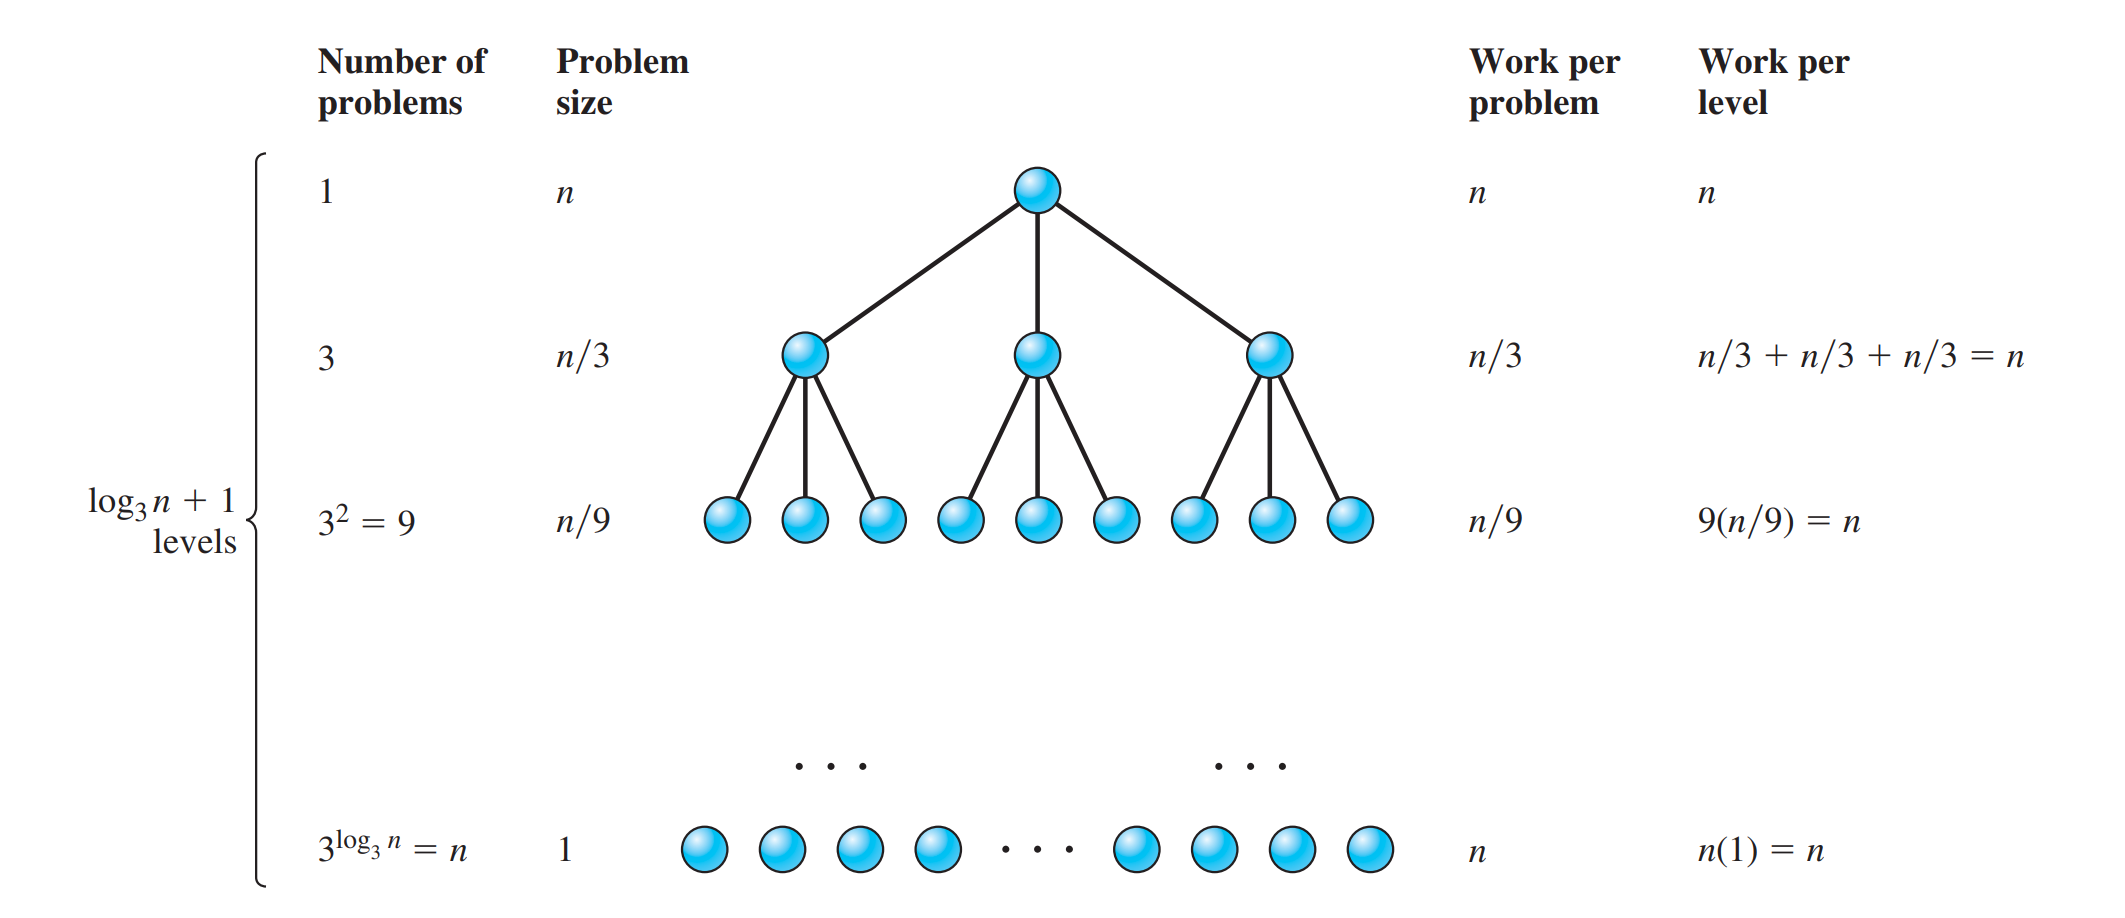
\includegraphics[width=10cm]  {tree.png}}
    \caption{\label{1} Tree}
  \end{figure}
  The recurrence is of the form
  $$T(n) = aT(n/2) + n$$
  According to the Lemma 4.7, $T(n) = \Theta (n^{\log _2a})$\\
  So here $T(n) = \Theta (n^{\log _23})$\\
  Proof:\\
  At Level $i$, we have $3^i$ nodes, each corresponding to a problem of size $n/2^i$, Thus, at Level $i$, the total amount of work is $3^i(n/2^i) = n(3/2)^i$ units. Summing over the $\log_2n$ levels, we obtain
  $$3^{log_2n}T(1)+n\sum ^{(\log n) - 1}_{i = 0}(\frac{3}{2})^i.$$
  The sum given by the summation sign is a geometric series. Therefore, because $3/2 \neq 1$, the sum will be big$\Theta$ of the largest term (see Theorem 4.4). Because a > 2, the largest term in this case is clearly the last one, namely, $n(3/2)^{(log n)−1}$. Applying rules of exponents and logarithms, we get that n times the largest term is
  $\begin{aligned}
      n\left(\frac{3}{2}\right)^{\left(\log _{2} n\right)-1} & =\frac{2}{3} \cdot \frac{n \cdot 3^{\log n}}{2^{\log _2n}} \\
                                                             & =\frac{2}{3} \cdot \frac{n \cdot 3^{\log _2n}}{n}          \\
                                                             & =\frac{2}{3} \cdot 3^{\log _2n}                            \\
                                                             & =\frac{2}{3}\left(2^{\log_2 3}\right)^{\log _2n}           \\
                                                             & =\frac{2}{3}\left(2^{\log _2n}\right)^{\log _23}           \\
                                                             & =\frac{2}{3} \cdot n^{\log _23}\end{aligned}$\\
  Thus, $T(1)3^{\log _2n} = T(1)n^{\log _23}$. Because $2/a$ and $T(1)$ are both nonnegative, the total work done is $\Theta(n^{\log _2 a})$.
\end{solution}
%%%%%%%%%%%%%%%

%%%%%%%%%%%%%%%
\begin{problem}[CS 4.3-18]
Suppose you are given recurrences of the form $T(n) = aT(n/b) + g(n)$, with $T(1) = d > 0$ and $g(n) > 0$ for all $n$, and $S(n) = aS(n/b) + g(n)$, with $S(1) = 0$ (and the same $a, b$, and $g(n)$). Is there any difference in the big behavior of the solutions to the two recurrences? What does this say about the influence of the initial condition on the big behavior of such recurrences?
\end{problem}

\begin{solution}
  $S(n) = \sum _{i = 0} ^{\log _b n-1} a^ig(\frac{n}{b^i})$\\
  $T(n) = \sum _{i = 0} ^{\log _b n-1} a^ig(\frac{n}{b^i}) + dn^{\log _b a}$\\
  Let $f(n) = \sum _{i = 0} ^{\log _b n-1} a^ig(\frac{n}{b^i})$\\
  If $n^{\log _b a} = O(f(n))$, then $S(n) = \Theta (T(n))$\\
  else if $n^{\log _b a} = \omega(f(n))$, then $S(n) = o(T(n))$, in this condition the initial condition has the influence on the big begavior of such recurrences.
\end{solution}
%%%%%%%%%%%%%%%

%%%%%%%%%%%%%%%
\begin{problem}[CS 4.5-8]
Show by induction that
$$
  T(n)= \begin{cases}8 T(n / 2)+n \log n & \text { if } n>1 \\ d & \text { if } n=1\end{cases}
$$
has $T(n) = O(n^3)$ for any solution $T(n)$
\end{problem}

\begin{solution}
  Bace Case: $T(1) = d$ and $T(n) = 8 T(n / 2)+n \log n$(if $n > 1$).\\
  Inductive hypothesis: $T(k) \leq ck^3 - k \log k(k < n)$.\\
  Inductive step:
  $\begin{aligned}
      T(n) & = 8 T(n / 2)+n \log n                                          \\
           & \leq 8(\frac{cn^3}{8} - \frac{n}{2}\log \frac{n}{2}) + n\log n \\
           & = cn^3 -3n\log n + 4n\log 2                                    \\
           & \leq cn^3 + n\log n(n >= 2)
    \end{aligned}$\\
  When $c > d$, the base case $T(1) = d$ also holds.\\
  Therefore, $T(n) = O(n^3)$
\end{solution}
%%%%%%%%%%%%%%%

%%%%%%%%%%%%%%%
\begin{problem}[CS 4.5-10]
Give the best big O upper bound you can for the solution to the recurrence
$$T(n) = 2T(\frac{n}{3} - 3) + n$$
(making an informed guess is not a bad idea here). Then prove by induction that your upper bound is correct.
\end{problem}

\begin{solution}
  $T(n) = O(n)$\\
  Proof:\\
  Assume that $T(n) \leq kn$\\
  $\begin{aligned}
      T(n) & = 2T(\frac{n}{3} - 3) + n    \\
           & \leq 2k(\frac{n}{3} - 3) + n \\
           & =(\frac{2}{3}k+1)n-6k        \\
           & \leq kn(k \geq 3)
    \end{aligned}$
\end{solution}
%%%%%%%%%%%%%%%

%%%%%%%%%%%%%%%%%%%%
\beginoptional

%%%%%%%%%%%%%%%
\begin{problem}[Linear Recurrences]
Give initial conditions $a_0$, $a_1$, and $a_2$ for which the growth rate of the solution to
\[
  a_{n} = 2a_{n-1} - a_{n-2} + 2a_{n-3} \quad \text{for } n > 2
\]
is (1) constant, (2) exponential, and (3) fluctuating in sign.
\end{problem}

\begin{solution}

\end{solution}
%%%%%%%%%%%%%%%

%%%%%%%%%%%%%%%%%%%%
\beginot

%%%%%%%%%%%%%%%
% \begin{ot}[]
% 
%   \noindent 参考资料:
%   \begin{itemize}
%     \item 更多精彩, 由你掌握。
%   \end{itemize}
% \end{ot}

% \begin{solution}
% \end{solution}
%%%%%%%%%%%%%%%
% \vspace{0.50cm}
%%%%%%%%%%%%%%%
本周两个 OT 介绍同一个重要主题: Generating Functions。
由每个班级的两位同学合作完成。

\begin{ot}[Generating Functions]
  介绍 Generating Functions 的概念、技巧与应用(包括但不限于它在解递归式中的应用)。

  \noindent 参考资料
  \begin{itemize}
    \item Section 7 of Book ``Concrete Mathematics'' by GKP~\cite{Book:GKP}
    \item \href{https://courses.csail.mit.edu/6.042/spring18/mcs.pdf}{Section 16 of Book ``Mathematics for Computer Science'' @ MIT, 2018}
    \item \href{https://en.wikipedia.org/wiki/Generating\_function}{Generating function @ wiki}
    \item 更多精彩, 由你掌握。
  \end{itemize}
\end{ot}

% \begin{solution}
% \end{solution}
%%%%%%%%%%%%%%%

%%%%%%%%%%%%%%%%%%%%
% 如果没有需要订正的题目,可以把这部分删掉

% \begincorrection
%%%%%%%%%%%%%%%%%%%%

%%%%%%%%%%%%%%%%%%%%
% 如果没有反馈,可以把这部分删掉
\beginfb

% 你可以写
% ~\footnote{优先推荐 \href{problemoverflow.top}{ProblemOverflow}}:
% \begin{itemize}
%   \item 对课程及教师的建议与意见
%   \item 教材中不理解的内容
%   \item 希望深入了解的内容
%   \item $\cdots$
% \end{itemize}
%%%%%%%%%%%%%%%%%%%%
\bibliography{2-5-solving-recurrence}
\bibliographystyle{plainnat}
%%%%%%%%%%%%%%%%%%%%
\end{document}